% !TeX root = RJwrapper.tex
\title{spinifex: An R Package for Creating a Manual Tour of Low-dimensional
Projections of Multivariate Data}
\author{by Nicholas Spyrison, Dianne Cook}

\maketitle

\abstract{%
Dynamic low-dimensional linear projections of multivariate data
collectively known as \textbf{tours} provide an important tool for
exploring multivariate data and models. The R package \pkg{tourr}
provides functions for several types of tours: grand, guided, little,
local and frozen. Each of these can be viewed dynamically, or saved into
a data object for animation. This paper describes a new package,
\pkg{spinifex}, to provide a manual tour, that allows the coefficient
for a single variable to be controlled. The variable is rotated fully
into the projection with a coefficient of 1 or -1, or completely out of
the projection with a coefficient of 0. The resulting sequence of
projections can be displayed using animation, with functions from either
the \pkg{plotly} and \pkg{gganimate} packages. By varying the
coefficient of a single variable, it is possible to explore the
sensitivity of structure in the projection to that variable. It is
particularly useful when used with a projection pursuit guided tour to
simplify and understand the solution. The use of the manual tour is
illustrated using a problem from particle physics.
}


\bibliography{spinifex_paper}

\hypertarget{introduction}{%
\section{Introduction}\label{introduction}}

Exploring multivariate spaces is a challenging task, increasingly so as
dimensionality increases. Traditionally, static low-dimensional
projections are used to display multivariate data in two dimensions,
such as principal component analysis, linear discriminant spaces or
projection pursuit. These are useful for finding relationships between
multiple variables, but they are limited because they show only a
glimpse of the high-dimensional space. An alternative approach is to use
a tour of dynamic linear projections, to look at many different
low-dimensional projections. Tours can be considered to extend the
dimensionality of visualization, which is important as data and models
exist in more than 3D. The package \CRANpkg{tourr} (Wickham et al.
\protect\hyperlink{ref-wickham_tourr_2011}{2011}) provides a platform
for generating tours. It has many types of tours available, and many
types of displays possible. A user can make a grand, guided, little,
local or frozen tour, and display the resulting projected data as a
scatterplot, density plot, histogram, or even as Chernoff faces if the
projection dimension is more than 3.

This work adds a manual tour to the collection. The manual tour was
described in Cook and Buja
(\protect\hyperlink{ref-cook_manual_1997}{1997}) and allows a user to
control the projection coefficients of a selected variable in a 2D
projection. The manipulation of these coefficients allows the analyst to
explore their sensitivity to the structure within the projection. As
manual tours operate on only one variable at a time, they are
particularly useful once a feature of interest has been identified.

One way to identify ``interesting'' features is with the use of a guided
tour (Cook et al. \protect\hyperlink{ref-cook_grand_1995}{1995}). Guided
tours select a very specific path, which approaches a projection that
optimizes an objective-function. The optimization is conducted in a
manner similar to simulated annealing (Kirkpatrick, Gelatt, and Vecchi
\protect\hyperlink{ref-kirkpatrick_optimization_1983}{1983}). The direct
optimization of a function allows guided tours to rapidly identify
interesting projection features given the relatively large
parameter-space. After a projection of interest is identified an analyst
can then use the ``finer brush'' of the manual tour, by controlling the
contributions of individual variables to explore the sensitivity they
have on the structure visible in the projection.

The paper is organized as follows. Section \ref{sec:algorithm} describes
the algorithm used to perform a radial manual tour as implemented in the
package \CRANpkg{spinifex}. Section \ref{sec:display} explains how to
generate an animation of the manual tour using the animation frameworks
offered by \CRANpkg{plotly} (Sievert
\protect\hyperlink{ref-sievert_plotly_2018}{2018}) and
\CRANpkg{gganimate} (Pedersen and Robinson
\protect\hyperlink{ref-pedersen_gganimate:_2019}{2019}). Package
functionality and code usage following the order applied in the
algorithm follows in section \ref{sec:usage}. Section
\ref{sec:application} illustrates how this can be used for sensitivity
analysis applied to multivariate data collected on high energy physics
experiments (Wang et al.
\protect\hyperlink{ref-wang_mapping_2018}{2018}). Section
\ref{sec:discussion} summarizes this paper and discusses potential
future directions.

\hypertarget{sec:algorithm}{%
\section{Algorithm}\label{sec:algorithm}}

The algorithm to conduct a manual tour interactively, by recording
mouse/cursor motion, is described in detail in Cook and Buja
(\protect\hyperlink{ref-cook_manual_1997}{1997}). Movement can be in any
direction and magnitude, but it can also be constrained in several ways:

\begin{itemize}
\tightlist
\item
  \emph{radial}: fix the direction of contribution, and allow the
  magnitude to change.
\item
  \emph{angular}: fix the magnitude, and allow the angle or direction of
  the contribution to vary.
\item
  \emph{horizontal}, \emph{vertical}: allow rotation only around the
  horizontal or vertical axis of the current 2D projection.
\end{itemize}

The algorithm described here produces a \textbf{radial} tour as an
\emph{animation sequence}. It takes the current contribution of the
chosen variable, and using rotation brings this variable fully into the
projection, completely removes it, and then returns to the original
position.

\hypertarget{notation}{%
\subsection{Notation}\label{notation}}

The notation used to describe the algorithm for a 2D radial manual tour
is as follows:

\begin{itemize}
\tightlist
\item
  \(\textbf{X}\), the data, an \(n \times p\) numeric matrix to be
  projected to 2D.
\item
  \(\textbf{B} = (B_1,~ B_2)\), any 2D orthonormal projection basis,
  \(p \times 2\) matrix, describing the projection from
  \(\mathbb{R}^p \Rightarrow \mathbb{R}^2\). This is called this the
  ``original projection'' because it is the starting point for the
  manual tour.
\item
  \(k\), is the index of the variable to manipulate, called the ``manip
  var''. 
\item
  \(\textbf{e}\), a 1D basis vector of length \(p\), with 1 in the
  \(k\)-th position and 0 elsewhere.
\item
  \(\textbf{M}\) is a \(p \times 3\) matrix, defining the 3D subspace
  where data rotation occurs, and is called the manip(ulation) space.
\item
  \(\theta\), the angle of in-projection-plane rotation, for example, on
  the reference axes; \(c_\theta, s_\theta\) are the cosine and sine.
\item
  \(\phi\), the angle of out-of-projection-plane rotation, into the
  manip space; \(c_\phi, s_\phi\) are the cosine and sine. The initial
  value for animation purposes is \(\phi_1\).
\item
  \(\textbf{U}\), the axis of rotation for out-of-projection rotation.
\item
  \(\textbf{R}\), the 3D rotation matrix, for performing unconstrained
  3D rotations within the manip space, \(\textbf{M}\). 
\end{itemize}

The algorithm operates entirely on projection bases, and incorporates
the data only when making the projected data plots.

\hypertarget{steps}{%
\subsection{Steps}\label{steps}}

\hypertarget{step-0-set-up}{%
\subsubsection{Step 0) Set up}\label{step-0-set-up}}

The flea data (Lubischew
(\protect\hyperlink{ref-lubischew_use_1962}{1962})), available in the
\pkg{tourr} package, is used to illustrate the algorithm. The data
contains 74 observations on 6 variables, which are physical measurements
made on beetles. Each observation belongs to one of three species.

An initial 2D projection basis must be provided. A suggested way to
start is to identify an interesting projection using a projection
pursuit guided tour. Here the holes index is used to find a 2D
projection of the flea data, which shows three separated groups. Figure
\ref{fig:step0} shows the initial projection of the data. The left panel
displays the projection basis (\(\textbf{B}\)), and can be used as a
visual guide of the magnitude and direction that each variable
contributes to the projection. The right panel shows the projected data,
\(\textbf{Y}_{[n,~2]} ~=~ \textbf{X}_{[n,~p]} \textbf{B}_{[p,~2]}\). The
colour and shape of points is mapped to the flea species. This plot is
made using the \code{view\_basis()} function in \CRANpkg{spinifex},
which generates a \CRANpkg{ggplot2} (Wickham
\protect\hyperlink{ref-wickham_ggplot2:_2016}{2016}) object.

\begin{Schunk}
\begin{figure}

{\centering 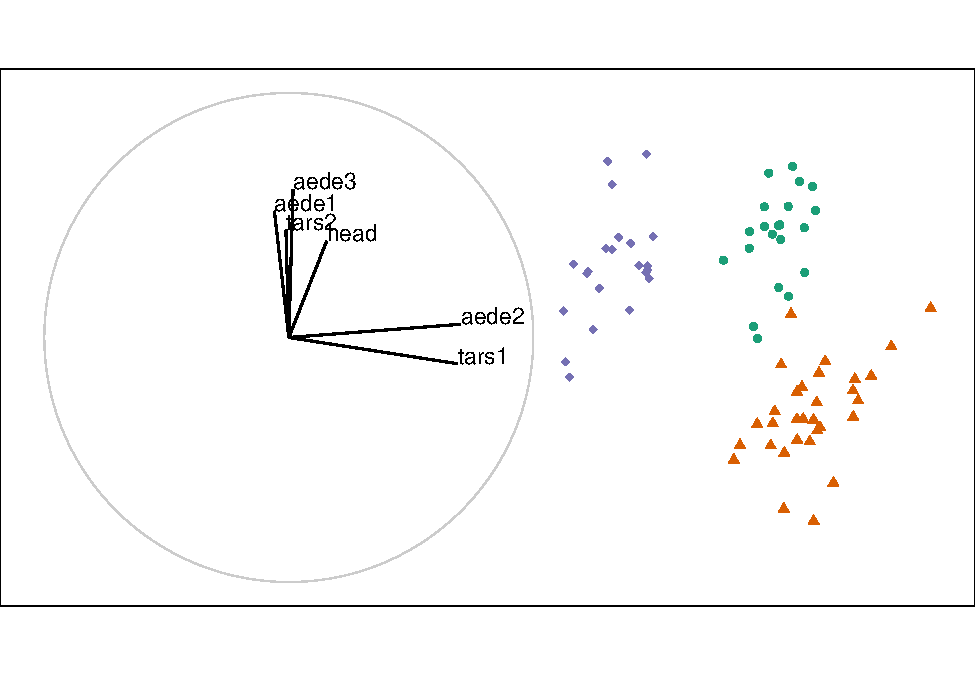
\includegraphics[width=0.7\linewidth]{spinifex_paper_files/figure-latex/step0-1} 

}

\caption[Initial 2D projection]{Initial 2D projection: representation of the basis  (left) and resulting data projection (right) of standardized flea data. The color and shape of data points are mapped to beetle species. The basis was identified using a projection pursuit guided tour, with the holes index. The contribution of the variables aede2 and tars1 approximately contrasts the other variables. The visible structure in the projection are the three clusters corresponding to the three species. Produced with the function \code{view\_basis()}.}\label{fig:step0}
\end{figure}
\end{Schunk}

\hypertarget{step-1-choose-manip-variable}{%
\subsubsection{Step 1) Choose manip
variable}\label{step-1-choose-manip-variable}}

In Figure \ref{fig:step0} the contribution of the variables tars1 and
aede2 mostly contrast the contribution of the other four variables.
These two variables combined contribute in the direction of the
projection where the purple cluster is separated from the other two
clusters. The variable aede2 is selected as the manip var, the variable
to be controlled in the tour. The question that will be explored, is,
how important this variable is to the separation of the clusters.

\hypertarget{step-2-create-the-3d-manip-space}{%
\subsubsection{Step 2) Create the 3D manip
space}\label{step-2-create-the-3d-manip-space}}

Initialize the coordinate basis vector as a zero vector \(\textbf{e}\)
of length \(p\), and set the \(k\)-th element to 1. In the example data,
aede2 is the fifth variable in the data, so \(k=5\), set \(e_5=1\). Use
a Gram-Schmidt process to orthonormalize the coordinate basis vector on
the original 2D projection to describe a 3D manip space, \(\textbf{M}\).

\begin{align*}
  e_k &\leftarrow 1 \\ 
  \textbf{e}^*   &\leftarrow \textbf{e} - \langle \textbf{e}, \textbf{B}_1 \rangle \textbf{B}_1 - \langle \textbf{e}, \textbf{B}_2 \rangle \textbf{B}_2 \\ 
  \textbf{M}_{[p,~3]} &= (\textbf{B}_1,\textbf{B}_2,\textbf{e}^*)
\end{align*}

The manip space provides a 3D projection from \(p\)-dimensional space,
where the coefficient of the manip var can range completely between
{[}0, 1{]}. 3D rotation can be used to rotate the manip variable
completely into or completely out of a 2D projection. Figure
\ref{fig:step2} illustrates this 3D manip space with the manip var
highlighted. This representation is produced by calling the
\code{view\_manip\_space()} function. This diagram is purely used to
help explain the algorithm.

\begin{Schunk}
\begin{figure}

{\centering 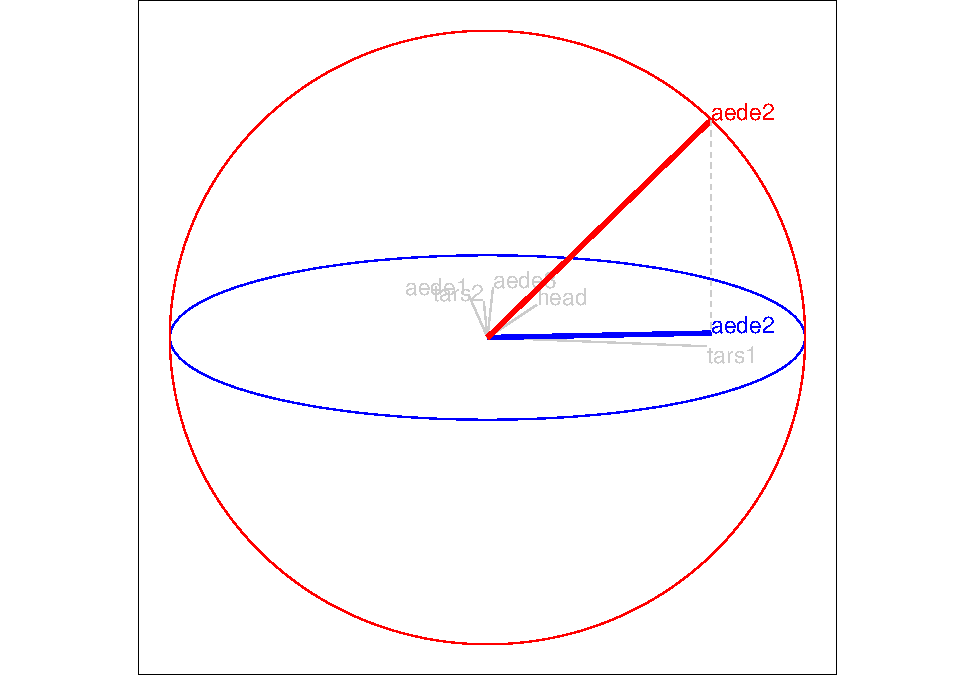
\includegraphics[width=0.7\linewidth]{spinifex_paper_files/figure-latex/step2-1} 

}

\caption[Illustration of a 3D manip space, constructed to change the contribution of the variable aede2 in the example data]{Illustration of a 3D manip space, constructed to change the contribution of the variable aede2 in the example data. The red circle indicates a unit sphere. The 2D projection is represented by the blue circle, with the projection coefficients represented by grey lines and text. The manip var axis, in red, has length 1 touching the sphere, extends the projection to a third dimension. The shadow of this axis (blue) is its contribution in the original 2D projection. Illustrated with the \code{view\_manip\_space()} function.}\label{fig:step2}
\end{figure}
\end{Schunk}

\hypertarget{step-3-defining-a-3d-rotation}{%
\subsubsection{Step 3) Defining a 3D
rotation}\label{step-3-defining-a-3d-rotation}}

The basis vector corresponding to the manip var (red line in Figure
\ref{fig:step2}), can be operated like a lever. This is the process of
the manual control, that rotates the manip variable into and out of the
2D projection (Figure \ref{fig:step3}). As the variable contribution is
controlled, the manip space rotates, and the projection onto the
horizontal projection plane correspondingly changes. This is a manual
tour. Generating a sequence of values for the rotation angles produces a
path for the rotation of the manip space.

For a radial tour, fix \(\theta\), the angle describing rotation within
the projection plane, and compute a sequence for \(\phi\), defining
movement out of the plane. This will change the initial value,
\(\phi_1\), the angle between \(\textbf{e}\) and its shadow in
\(\textbf{B}\), to a maximum of \(0\) (manip var fully in projection),
then to a minimum of \(\pi/2\) (manip var out of projection), before
returning to \(\phi_1\).

Rotations in 3D can be defined by the axes they pivot on. Rotation
within the projection, \(\theta\), is rotation around the \(Z\) axis.
Out-of-projection rotation, \(\phi\), is the rotation around an axis on
the \(XY\) plane, \(\textbf{U}\), orthogonal to \(\textbf{e}\). Given
these axes, the rotation matrix, \(\textbf{R}\) can be written as
follows, using Rodrigues' rotation formula (originally pubished in
Rodrigues (\protect\hyperlink{ref-rodrigues_lois_1840}{1840})):

\begin{align*}
    \textbf{R}_{[3,~3]} 
    &= \textbf{I}_3 + s_\phi\*\textbf{U} + (1-c_\phi)\*\textbf{U}^2 \\
        &=
    \begin{bmatrix}
      1&0&0 \\ 
      0&1&0 \\ 
      0&0&1 \\
    \end{bmatrix} +
    \begin{bmatrix}
      0 & 0 & c_\theta s_\phi \\
      0 & 0 & s_\theta s_\phi \\
      -c_\theta s_\phi & -s_\theta s_\phi & 0 \\
    \end{bmatrix} +
    \begin{bmatrix}
      -c_\theta (1-c_\phi) & s^2_\theta (1-c_\phi) & 0 \\
      -c_\theta s_\theta (1-c_\phi) & -s^2_\theta (1-c_\phi) & 0 \\
      0 & 0 & c_\phi-1 \\
    \end{bmatrix} \\
    &= 
    \begin{bmatrix}
      c_\theta^2 c_\phi + s_\theta^2 &
      -c_\theta s_\theta (1 - c_\phi) &
      -c_\theta s_\phi \\
      -c_\theta s_\theta (1 - c_\phi) &
      s_\theta^2 c_\phi + c_\theta^2 &
      -s_\theta s_\phi \\
      c_\theta s_\phi &
      s_\theta s_\phi &
      c_\phi
    \end{bmatrix} \\
\end{align*}

\noindent where

\begin{align*}
  \textbf{U} &= (u_x, u_y, u_z) =
  (s_\theta, -c_\theta, 0) \\ 
  &=
  \begin{bmatrix}
  0 & -u_z & u_y  \\
  u_z & 0 & -u_x \\
  -u_y & u_x & 0 \\
  \end{bmatrix} =
  \begin{bmatrix}
    0 & 0 & -c_\theta \\
    0 & 0 & -s_\theta \\
    c_\theta & s_\theta & 0 \\
  \end{bmatrix} \\
  \end{align*}

\hypertarget{step-4-creating-an-animation-of-the-radial-rotation}{%
\subsubsection{Step 4) Creating an animation of the radial
rotation}\label{step-4-creating-an-animation-of-the-radial-rotation}}

The steps outlined above can be used to create any arbitrary rotation in
the manip space. To use these for sensitivity analysis, the radial
rotation is built into an animation where the manip var is rotated fully
into the projection, completely out, and then back to the initial value.
This involves allowing \(\phi\), to vary between 0 and \(\pi/2\), call
the steps \(\phi_i\).

\begin{Schunk}
\begin{figure}

{\centering 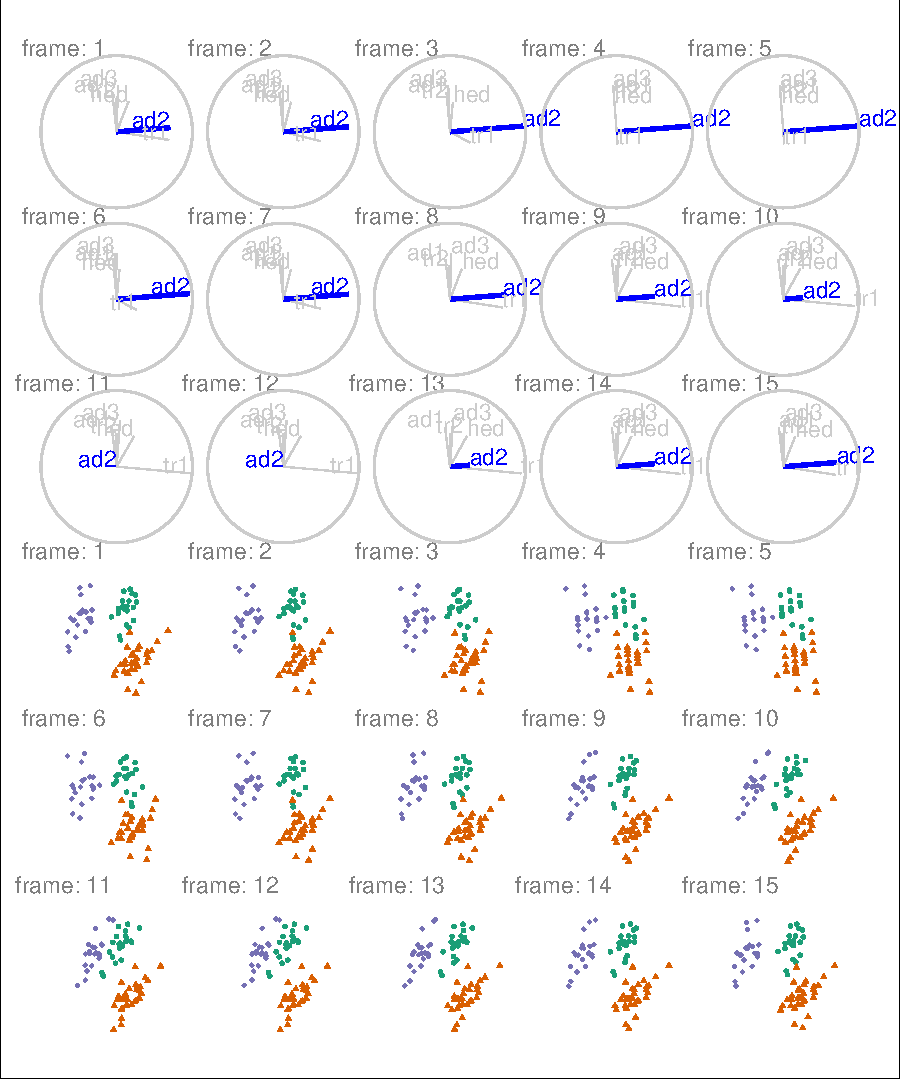
\includegraphics[width=1\linewidth]{spinifex_paper_files/figure-latex/step3-1} 

}

\caption[Snapshots of a radial manual tour manipulating aede2]{Snapshots of a radial manual tour manipulating aede2: (1) original projection, (2) full contribution, (3) zero contribution, (4) back to original. }\label{fig:step3}
\end{figure}
\end{Schunk}

\begin{enumerate}
\def\labelenumi{\arabic{enumi}.}
\tightlist
\item
  Set initial value of \(\phi_1\) and \(\theta\):
  \(\phi_1 = \cos^{-1}{\sqrt{B_{k1}^2+B_{k2}^2}}\),
  \(\theta=\tan^{-1}\frac{B_{k2}}{B_{k1}}\). \(\phi_1\) is the angle
  between \(\textbf{e}\) and its shadow in \(\textbf{B}\). Check that
  \(\phi_1\) is between 0 and \(\pi/2\), and if not, transform it into
  this range, by subtracting or adding \(\pi\). (XXX Nick needs to check
  this math, and the ways to check and fix if angle produced by the
  calculation given fall in the right range.)
\item
  Set an angle increment (\(\Delta_\phi\)) that sets the step size for
  the animation, to rotate the manip var into and out of the projection.
  (Note: Using angle increment, rather than a number of steps, to
  control the movement, is consistent with the tour algorithm as
  implemented in the \pkg{tourr}).
\item
  Step towards \(0\), where the manip var is a completely in the
  projection.
\item
  Step towards \(\pi/2\), where the manip variable has no contribution.
\item
  Step back to \(\phi_1\).
\end{enumerate}

In each of the steps 3-5, a small step may be added to ensure that the
end points of \(\phi\) (0, \(\pi/2\)) are reached.

\hypertarget{sec:display}{%
\subsubsection{Step 4) Projecting the data}\label{sec:display}}

The operation of a manual tour is defined on the projection bases. Only
when the data plot needs to be made is the data projected into the
relevant basis.

\begin{align*}
  \textbf{Y}_{[n,~3]} &= \textbf{X}_{[n,~p]} \textbf{M}_{[p,~3]} \textbf{R}^{(i)}_{[3,3]}
\end{align*}

\noindent where \(\textbf{R}^{(i)}_{[3,3]}\) is the incremental rotation
matrix, using \(\phi_i\). To make the data plot, use the first two
columns of \textbf{Y}. Show the projected data for each frame in
sequence to form an animation.

Figure \ref{fig:step4} illustrates a manual tour sequence having 15
steps. The projection axes are displayed on the top half, which
correspond to the projected data in the bottom half. When aede2 is
removed from the projection, the purple cluster overlaps with the green
cluster. This suggests that aede2 is important for distinguishing this
species.

Tours are typically viewed as an animation. The animation of this tour
can be viewed online at
\url{https://nspyrison.netlify.com/thesis/flea_manualtour_mvar5/}. The
page may take a moment to load. Animations can be produced using the
function \code{play\_manual\_tour()}.

\begin{Schunk}
\begin{figure}

{\centering 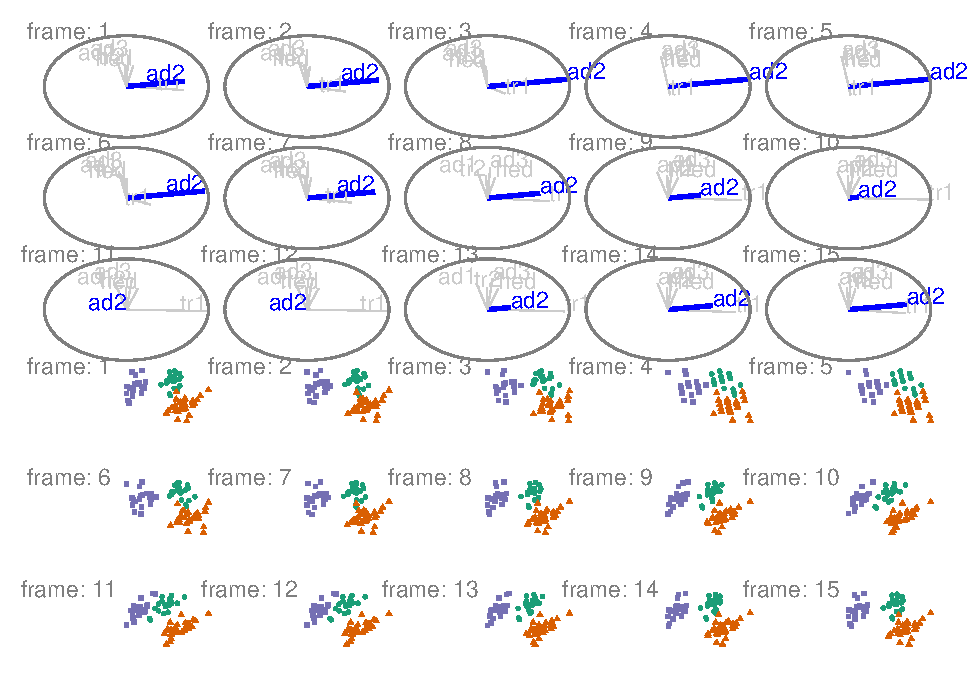
\includegraphics[width=5.83in,height=7in]{spinifex_paper_files/figure-latex/step4-1} 

}

\caption[Radial manual tour manipulating aede2 of standardized flea data]{Radial manual tour manipulating aede2 of standardized flea data. The axis for aede2 increases in contribution to the projection, from its initial value to 1, decreasing to 0 and then returning to the initial value. This affects the separatiion between the purple and green clusters. This shows that aede2 is important for distinguishing the purple species, because the separation disappears when aede2 is not contributing to the projection. An animation can be viewed at https://nspyrison.netlify.com/thesis/flea\_manualtour\_mvar5/.}\label{fig:step4}
\end{figure}
\end{Schunk}

\hypertarget{sec:usage}{%
\section{Package structure and functionality}\label{sec:usage}}

This section describes the functions available in the package, and how
to use them.

\hypertarget{installation}{%
\subsection{Installation}\label{installation}}

The \CRANpkg{spinifex} is available from CRAN, and can be installed by:

\begin{Schunk}
\begin{Sinput}
install.package("spinifex")
library("spinifex")
\end{Sinput}
\end{Schunk}

\noindent Also see the vignette for examples of usage:

\begin{verbatim}
vignette("spinifex_vignette")
\end{verbatim}

\noindent The development version can be installed from github:

\begin{verbatim}
remotes::install_github("nspyrison/spinifex") 
\end{verbatim}

\hypertarget{functions}{%
\subsection{Functions}\label{functions}}

Table \ref{tab:functionsTable} lists the primary functions and their
purpose. These are grouped into four types: construction for building a
tour path, render to make the plot objects, animation for running the
animation, and specialty for providing illustrations used in the
algorithm description.

\begin{Schunk}
\begin{table}[t]

\caption{\label{tab:functionsTable}Summary of available functions.}
\centering
\begin{tabular}{lll}
\toprule
Class & Function & Description\\
\midrule
construction & create\_manip\_space & forms the 3D space of rotation\\
construction & rotate\_manip\_space & performs 3D rotation\\
construction & manual\_tour & generates sequence of 2D frames\\
 &  & \\
render & render\_ & constructs the ggplot object to feed to animation\\
render & render\_plotly & converts the ggplot object to a plotly animation\\
render & render\_gganimate & converts the ggplot object to a gganimate  animation\\
render & array2df & turns a tour path array into long form, for plotting\\
 &  & \\
animation & play\_tour\_path & animates given tour path\\
animation & play\_manual\_tour & animates the manual tour algorithm\\
 &  & \\
specialty & view\_basis & displays the reference frame of a given basis\\
specialty & view\_manip\_space & illustrative display of any manip space\\
\bottomrule
\end{tabular}
\end{table}

\end{Schunk}

\hypertarget{algorithm-code}{%
\subsection{Algorithm code}\label{algorithm-code}}

We'll start by initializing values including a standardized data set
(numeric columns only), a starting basis, a categorical variable for
point aesthetics (optional), and a manip var. To get bearings on the
projection, start by observing the reference axes of the basis with
\code{view\_basis()} producing Figure \ref{fig:step0}.

\begin{Schunk}
\begin{Sinput}
f_data  <- tourr::rescale(flea[, 1:6])                    ## standardize data
f_path  <- save_history(f_data, guided_tour(holes()))     ## produce guided tour
f_basis <- matrix(f_path[,, max(dim(f_path)[3])], ncol=2) ## end of guided tour
f_cat   <- factor(flea$species)                           ## categorical var

view_basis(basis = f_basis, 
           data = f_data,
           labels = colnames(f_data))
\end{Sinput}
\end{Schunk}

After becoming familiar with this space, select a manip var, the
variable to change the contributions of. Use \code{view\_manip\_space()}
to view the new space with a dimension orthogonal to the projection
plane where the manip var has a full contribution. This illustrates how
the manip var is manipulated with the addition of the manip space as
shown in Figure \ref{fig:step2}.

\begin{Schunk}
\begin{Sinput}
f_mvar  <- 5  ## manip var number

view_manip_space(basis = f_basis, 
                 manip_var = f_mvar, 
                 labels = colnames(f_data))
\end{Sinput}
\end{Schunk}

Now we are ready to perform a manual tour on the selected variable. Use
\code{play\_manual\_tour()} to perform the algorithm as discussed above,
in section \ref{sec:algorithm}. This is the animated equivalent of
Figure \ref{fig:step3}.

\begin{Schunk}
\begin{Sinput}
angle_speed <- .26

play_manual_tour(data = f_data,
                 basis = f_basis, 
                 manip_var = f_mvar, 
                 angle = angle_speed,
                 col = f_cat,
                 pch = f_cat)
\end{Sinput}
\end{Schunk}

This concludes the content of the algorithm section, however, lets cover
animating paths generated in \pkg{tourr}. Animate the previously
generated guided tour path via \code{play\_tour\_path()}. Utility
functions can also be passed as arguments into either of the tour
animation function to change the resulting graphics object, set
\code{render\_type = render\_gganimate} to view the animation as a GIF.

\begin{Schunk}
\begin{Sinput}
play_tour_path(tour_path = f_path,
               data = f_data,
               render_type = render_gganimate, 
               angle = angle_speed
)
\end{Sinput}
\end{Schunk}

\hypertarget{rendering-and-sharing}{%
\subsection{Rendering and sharing}\label{rendering-and-sharing}}

The \pkg{tourr} package utilizes \pkg{base} graphics for the display of
tours. \pkg{spinifex} allows tours to be rendered in \pkg{plotly} as an
HTML5 object or \pkg{gganimate} as GIF or MP4 files. Sharing of
animations is not trivial, especially static formats like print and PDF.
Even with dynamic display capturing the correct resolution and aspect
ratio can be challenging, while many formats quickly bloat file sizes
limiting sharing options. Keep in mind hosting options and exporting
functions offered in \pkg{plotly}, \pkg{gganimate} and \pkg{tourr}.

\hypertarget{storage}{%
\subsection{Storage}\label{storage}}

Storing each data point for every frame of the animation is redundant.
Just as operations are performed on the bases, so too should tour paths
be stored as bases and a single instance of the data. Consider a radial
manual tour, we can store the salient features in 3 bases, where
\(\phi\) is at its starting, minimum, and maximum values. The frames in
between can be interpolated by supplying angular speed. With the use of
the \code{tourr::save\_history()} function, the target bases can be
saved. From there geodesic interpolation can be used to populate the
intermittent frames. This type of interpolation should not be used on
manual tours, which have already been initialized into a 3D manip space
where direct linear interpolation is appropriate.

\hypertarget{sec:application}{%
\section{Application}\label{sec:application}}

In a recent paper, Wang et al.
(\protect\hyperlink{ref-wang_mapping_2018}{2018}), the authors aggregate
and visualize the sensitivity of hadronic experiments to nucleon
structure. The authors introduce a new tool, PDFSense, to aid in the
visualization of parton distribution functions (PDF). The
parameter-space of these experiments lies in 56 dimensions,
\(\delta \in \mathbb{R}^{56}\), and are visualized as 3D subspaces of
the 10 first principal components in linear (PCA) and non-linear (t-SNE)
embeddings.

Using the same data, another study, Cook, Laa, and Valencia
(\protect\hyperlink{ref-cook_dynamical_2018}{2018}), applied grand tours
(Asimov \protect\hyperlink{ref-asimov_grand_1985}{1985}) to the same
subspaces. Grand tours are dynamic linear projections of high
dimensional spaces where basis sets are selected at random and animated
with geodesic interpolation of the intermediate frames. Because of the
change in the basis, or orientation to the subspace, tours are able to
better resolve the distribution shape of clusters, intra-cluster detail,
and better outlier detection than the use of PDFSense \& TFEP
(TensorFlow embedded projections) or traditional static embeddings.
Before applying manual tours the structure of the data is discussed.

The data has a hierarchical structure with top-level clusters; DIS, VBP,
and jet. Each cluster is a particular class of experiments, each with
many experimental datasets which, in turn, have many observations. In
consideration of data density, we conduct manual tours on subsets of the
DIS and jet clusters. This explores the sensitivity of the structure to
each of the variables in turn and we present the subjectively best and
worst variable to manipulate for identifying dimensionality of the
clusters and describing the span of the clusters.

\hypertarget{jet-cluster}{%
\subsection{Jet cluster}\label{jet-cluster}}

The jet cluster resides in a smaller dimensionality than the full set of
experiments with four principal components explaining 95\% of the
variation in the cluster (Cook, Laa, and Valencia
\protect\hyperlink{ref-cook_dynamical_2018}{2018}). The data within this
4D embedding is subset down to ATLAS7old and ATLAS7new to focus in on
two groups with a reasonable number of observations that occupy
different parts of the subspace. Radial manual tours controlling
contributions from PC4 and PC3 are shown in Figure
\ref{fig:JetClusterGood} and Figure \ref{fig:JetClusterBad}
respectively. These variables are selected to contrast the information
conveyed by different manip variables. Links to dynamic HTML5 animations
controlling each of the four variables are also provided.

When manipulating PC4, there is a clear difference in the parameter
space spanned by the experiment types ATLAS7new and ATLAS7old.
Specifically, the variation of ATLAS7new (green) becomes more singular.
The experiments are probing different parameter space and PC4 is
important to demonstrate this. Yet, when PC3 is manipulated there is no
clear indication that the different experiments probe different
parameter space. Performing a radial manual tour on PC4 is more
insightful than for PC3. Radial manual tours manipulating each of the
principal components in the jet cluster can be viewed by following the
links:
\href{https://nspyrison.netlify.com/thesis/jetcluster_manualtour_pc1/}{PC1},
\href{https://nspyrison.netlify.com/thesis/jetcluster_manualtour_pc2/}{PC2},
\href{https://nspyrison.netlify.com/thesis/jetcluster_manualtour_pc3/}{PC3},
and
\href{https://nspyrison.netlify.com/thesis/jetcluster_manualtour_pc4/}{PC4}.

\begin{Schunk}
\begin{figure}

{\centering 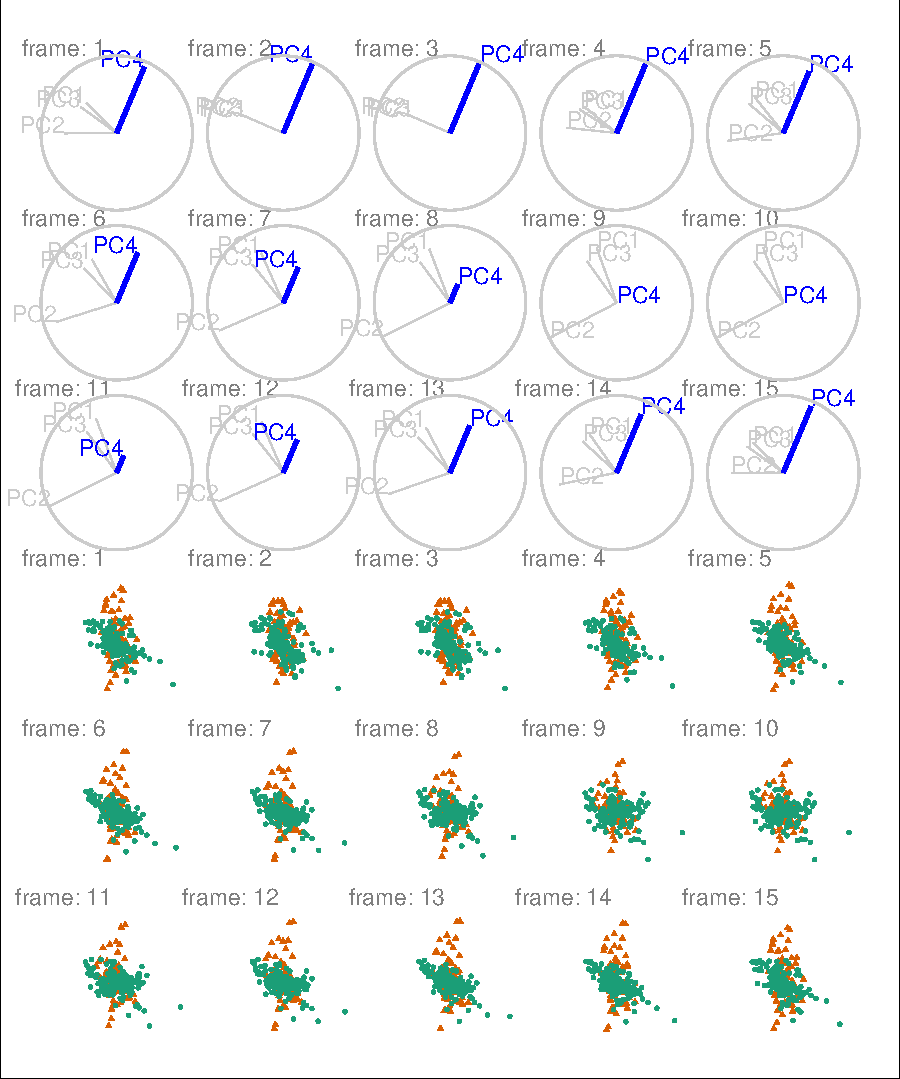
\includegraphics[width=5.83in,height=7in]{spinifex_paper_files/figure-latex/JetClusterGood-1} 

}

\caption[A radial manual tour of PC4 within the jet cluster]{A radial manual tour of PC4 within the jet cluster. Colored by experiment type: ATLAS7new in green and ATLAS7old in orange. When PC4 fully/negligibly contributes to the projection ATLAS7new (green) spans the same space as the orange points. During the intermediate frames, the ATLAS7new is compressed in the direction radial to PC4. The differece in distribution shape demonstrates the experiments probe different phase-space, which has a linear mapping back to the original variables for interpretation and further exploration. An HTML5 version can be viewed at https://nspyrison.netlify.com/thesis/jetcluster\_manualtour\_pc4/.}\label{fig:JetClusterGood}
\end{figure}
\end{Schunk}

\begin{Schunk}
\begin{figure}

{\centering 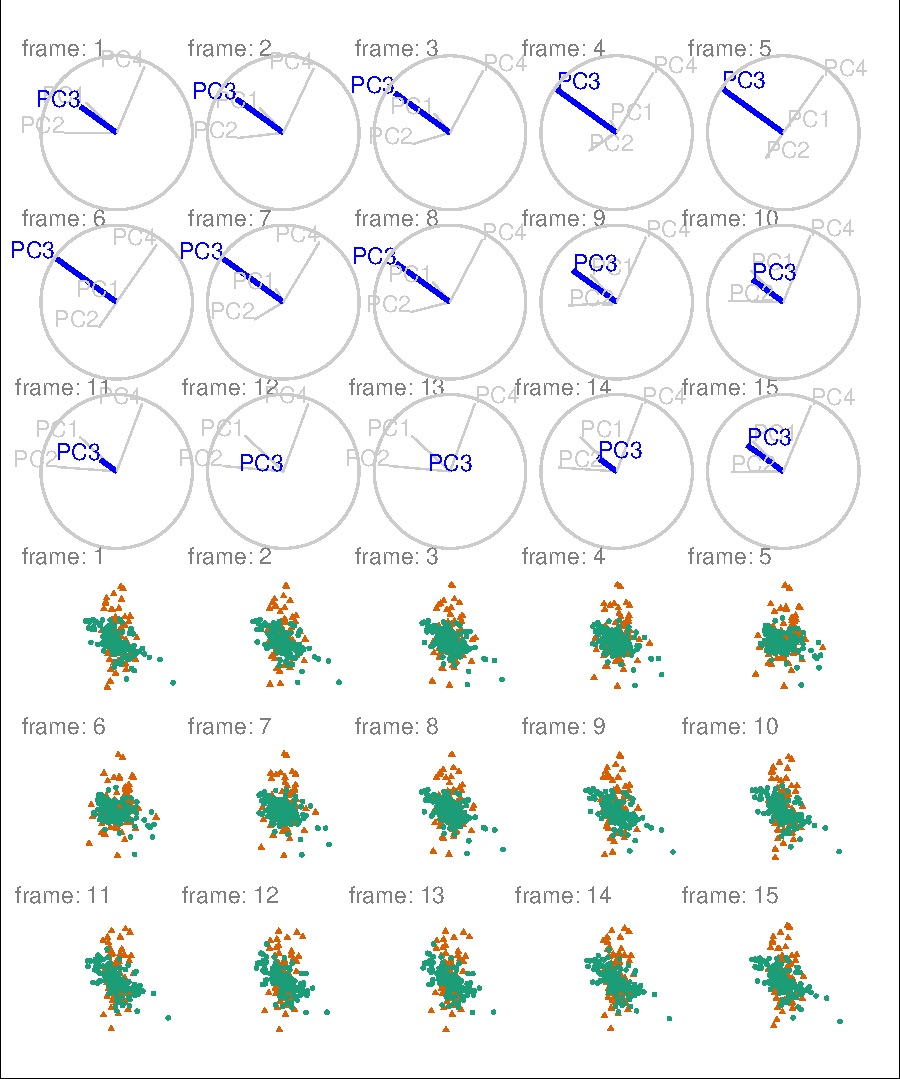
\includegraphics[width=5.83in,height=7in]{spinifex_paper_files/figure-latex/JetClusterBad-1} 

}

\caption[A radial manual tour of PC4 within the jet cluster]{A radial manual tour of PC4 within the jet cluster. Colored by experiment type: ATLAS7new in green and ATLAS7old in orange. Data from ATLAS7new (green) spans mostly the same space as ALTLAS7old (orange) with no evident difference in cluster structure across varying contributions of PC3. An HTML5 version can be viewed at https://nspyrison.netlify.com/thesis/jetcluster\_manualtour\_pc3/.}\label{fig:JetClusterBad}
\end{figure}
\end{Schunk}

\hypertarget{dis-cluster}{%
\subsection{DIS cluster}\label{dis-cluster}}

A different space is used to explore the DIS cluster; specifically the
first six principal components, which explains 48\% of the variation
contained within the aggregated data (Cook, Laa, and Valencia
\protect\hyperlink{ref-cook_dynamical_2018}{2018}). Radial manual tours
are performed on PC6 and PC2 in Figure \ref{fig:DISclusterGood} and
Figure \ref{fig:DISclusterBad} respectively.

The selection of the manip variable is important, as the manip spaces
convey substantially different information. The manual tour of PC6
offers information about the dimensionality, shape, and orientations of
the different experiment classes. PC6 is particularly important to
describe the variations of DIS HERA1+2 and charm SIDIS observations,
Whereas manipulating the contributions of PC2 only shows a subset of the
dimensionality and shape information. Manipulating the contributions of
PC6 turned out to be much more insightful than PC2. This result might
seem counter-intuitive at first as PC2 should explain much more of the
variation in the data. However, features and structures in the data
regularly reside in smaller dimensionality which can be overlooked when
optimizing on full sample statistics. DIS cluster manual tours
manipulating each of the principal components can be viewed from the
links:
\href{https://nspyrison.netlify.com/thesis/discluster_manualtour_pc1/}{PC1},
\href{https://nspyrison.netlify.com/thesis/discluster_manualtour_pc2/}{PC2},
\href{https://nspyrison.netlify.com/thesis/discluster_manualtour_pc3/}{PC3},
\href{https://nspyrison.netlify.com/thesis/discluster_manualtour_pc4/}{PC4},
\href{https://nspyrison.netlify.com/thesis/discluster_manualtour_pc5/}{PC5},
and
\href{https://nspyrison.netlify.com/thesis/discluster_manualtour_pc6/}{PC6}.

\begin{Schunk}
\begin{figure}

{\centering 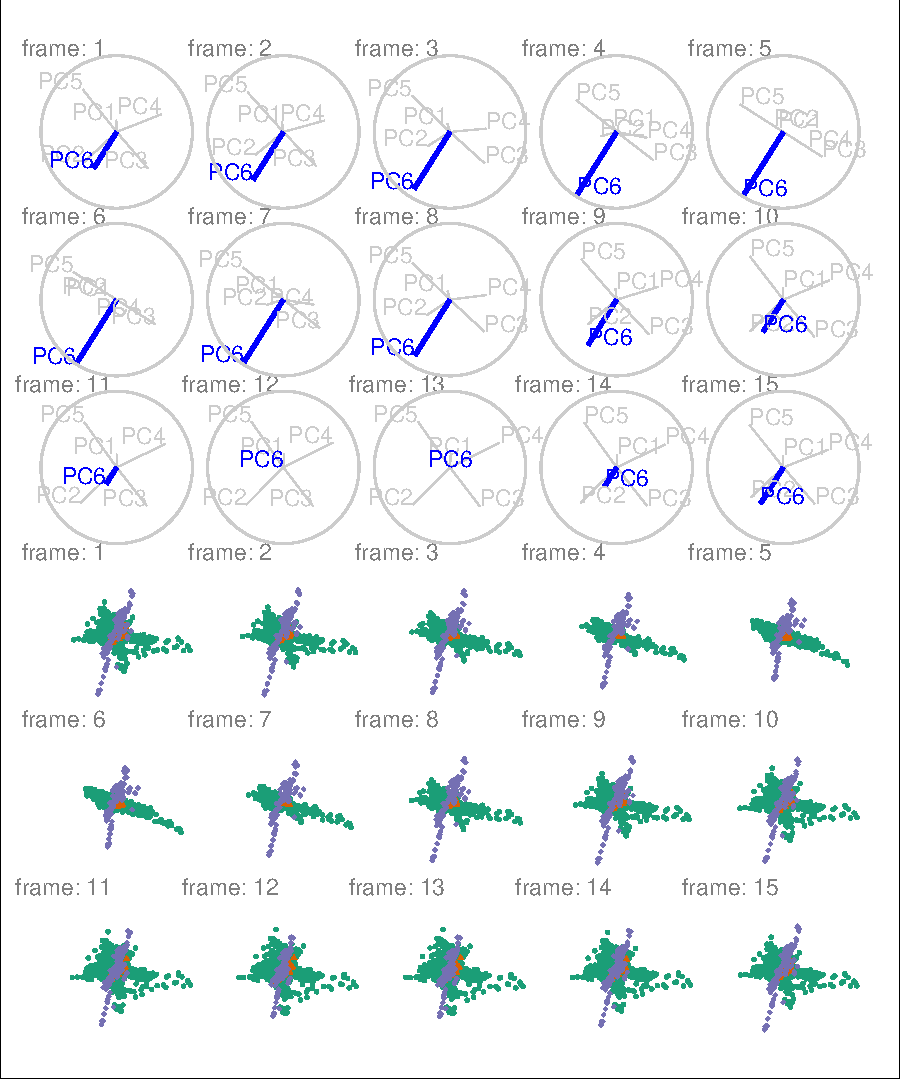
\includegraphics[width=5.83in,height=7in]{spinifex_paper_files/figure-latex/DISclusterGood-1} 

}

\caption[A radial manual tour manipulating the contribution of PC6 within the DIS cluster]{A radial manual tour manipulating the contribution of PC6 within the DIS cluster. Points are colored by experiment type: DIS HERA1+2 in green, dimuon SIDIS in purple, and charm SIDIS in orange. The cluster DIS HERA1+2 (green) is distributed in a cross-shaped plane, charm SIDIS (orange) occupies the center space of this cross. As the contribution of PC6 becomes whole the distributions of DIS HERA1+2 (green) and charm SIDIS (orange) become singular but offset by a small angle. Less evident is the linear dimuon SIDIS (purple) observations approaching the line of view for intermediate values of PC6. An HTML5 version can be viewed at https://nspyrison.netlify.com/thesis/discluster\_manualtour\_pc6/.}\label{fig:DISclusterGood}
\end{figure}
\end{Schunk}

\begin{Schunk}
\begin{figure}

{\centering 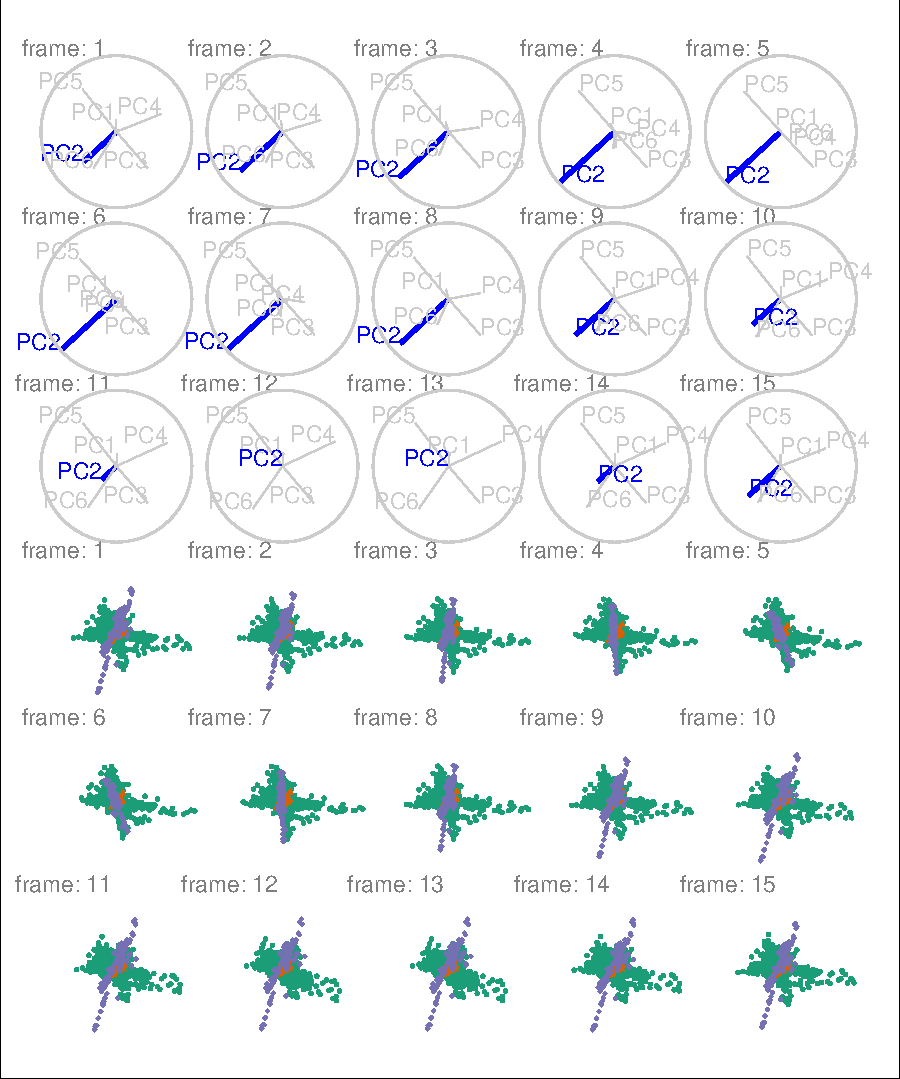
\includegraphics[width=5.83in,height=7in]{spinifex_paper_files/figure-latex/DISclusterBad-1} 

}

\caption[A radial manual tour manipulating the contribution of PC2 within the DIS cluster]{A radial manual tour manipulating the contribution of PC2 within the DIS cluster. Points are colored by experiment type: DIS HERA1+2 in green, dimuon SIDIS in purple, and charm SIDIS in orange. The plane of cross distributed DIS HERA data (green) and a nearly orthogonal jet of dimuon SIDIS (purple) is present. This jet does extend more in the plane of view when the contribution of PC2 is full, giving insight to its orientation. However, less information about the shape of DIS HERA (green) and charm SIDIS (orange) is available compared to PC6 as the manip var. An HTML5 version can be viewed at https://nspyrison.netlify.com/thesis/discluster\_manualtour\_pc2/.}\label{fig:DISclusterBad}
\end{figure}
\end{Schunk}

\hypertarget{sec:discussion}{%
\section{Discussion}\label{sec:discussion}}

Tours, which are a dynamic linear projection of numeric multivariate
data, play an important role in data visualization; they extend the
dimensionality of visuals while data- and parameter-spaces become ever
larger. This research has modified the algorithm producing manual tours
which and has made this functionality available in package
\pkg{spinifex}. The package adds to \pkg{tourr}, extending the graphics
offerings that can be used to display tours.

Radial manual tours were applied to a dataset across different
experiments of hadronic collisions. The importance of selecting the
correct manip var, as demonstrated by comparing tours of varying amounts
of structural information. Manual tours, by controlling the contribution
of the manip var on the projection, enable analysts to explore the
sensitivity that variable has on the structure of the projection. This
information can be used by domain experts to identify which variables
are probing which parameter spaces and how sensitive structural features
are to different variables. This insight can be indispensable for
variable inclusion/exclusion, and in higher-level decisions, such as
meta-analysis, to suggest directions of future research.

Future research on the algorithm would include extending it for use in
3D projections. The addition of another dimension theoretically allows
for improved perception. In some frameworks, such as the game engine
\textbf{unity}, this would allow for the exploration in immersive
virtual reality or mixed reality, which may further allow for a better
perception of structure and aid in higher-dimensional function
visualization. Functions with many parameters suffer from the same
dimensionality problem as data while their possible values lie on a
surface of values rather than discrete points. Occulation, or the closer
surface blocking further surfaces, will likely be an issue that may be
alleviated by the use of wire mesh, changing opacity, or looking at
sections of the projections known as prosections (Furnas and Buja
\protect\hyperlink{ref-furnas_prosection_1994}{1994}).

The \pkg{tourr} package provides many other geometric displays with the
\code{tourr::display\_*()} family. These geometric options could be
integrated into the \pkg{ggplot2} framework for display on \pkg{plotly}
and \pkg{gganimate}. Additionally, the \CRANpkg{animation} package Xie
et al. (\protect\hyperlink{ref-xie_animation:_2018}{2018}) could be
implemented for another graphics framework. However, \pkg{animation}
builds from \pkg{base} graphics while \pkg{spinifex} utilizes
\pkg{ggplot2} graphics, a significant paradigm shift, which may have a
low return on investment.

The Givens rotations and Householder reflections as outlined in Buja et
al. (\protect\hyperlink{ref-buja_computational_2005}{2005}) could also
be added. Currently, Gram-Schmidt is the only form of frame
interpolation used. In a Givens rotation, the \(x\) and \(y\) components
(for example \(\theta~= 0,~pi/2\)) of the in-plane rotation are
calculated separately and would be applied sequentially to produce the
radial rotation. Householder reflections define reflection axes to
project points on to the axes to generate rotations.

Having script-only interaction with tours causes a significant barrier
to entry. To a lesser extent, \pkg{plotly} offers some static
interactions with the contained object, such as tooltips, brushing, and
linking without communicating back to the R console. The development of
a dynamic graphical user interface, perhaps with the use of a
\CRANpkg{shiny} (Chang et al.
\protect\hyperlink{ref-chang_shiny:_2018}{2018}) application, would
mitigate the barrier to entry, allow for more rapid analysis, and offer
an approachable demo tool. The user could easily switch between
variables to control, adjust the interpolation step angle, or flag/save
specific frame basis sets.

\hypertarget{acknowledgments}{%
\section{Acknowledgments}\label{acknowledgments}}

This article was created in R (R Core Team
\protect\hyperlink{ref-r_core_team_r:_2018}{2018}), using
\CRANpkg{knitr} (Xie \protect\hyperlink{ref-stodden_knitr:_2014}{2014})
and \CRANpkg{rmarkdown} (Xie, Allaire, and Grolemund
\protect\hyperlink{ref-xie_r_2018}{2018}), with code generating the
examples inline. The source files for this article be found at
\href{https://github.com/nspyrison/spinifex_paper/}{github.com/nspyrison/spinifex\_paper/}.
The source code for the \pkg{spinifex} package can be found at
\href{https://github.com/nspyrison/spinifex/}{github.com/nspyrison/spinifex/}.

\hypertarget{bibliography}{%
\section*{Bibliography}\label{bibliography}}
\addcontentsline{toc}{section}{Bibliography}

\hypertarget{refs}{}
\leavevmode\hypertarget{ref-asimov_grand_1985}{}%
Asimov, Daniel. 1985. ``The Grand Tour: A Tool for Viewing
Multidimensional Data.'' \emph{SIAM Journal on Scientific and
Statistical Computing} 6 (1): 128--43.
\url{https://doi.org/https://doi.org/10.1137/0906011}.

\leavevmode\hypertarget{ref-buja_computational_2005}{}%
Buja, Andreas, Dianne Cook, Daniel Asimov, and Catherine Hurley. 2005.
``Computational Methods for High-Dimensional Rotations in Data
Visualization.'' In \emph{Handbook of Statistics}, 24:391--413.
Elsevier. \url{https://doi.org/10.1016/S0169-7161(04)24014-7}.

\leavevmode\hypertarget{ref-chang_shiny:_2018}{}%
Chang, Winston, Joe Cheng, J. J. Allaire, Yihui Xie, and Jonathan
McPherson. 2018. \emph{Shiny: Web Application Framework for R}.
\url{https://CRAN.R-project.org/package=shiny}.

\leavevmode\hypertarget{ref-cook_manual_1997}{}%
Cook, Dianne, and Andreas Buja. 1997. ``Manual Controls for
High-Dimensional Data Projections.'' \emph{Journal of Computational and
Graphical Statistics} 6 (4): 464--80.
\url{https://doi.org/10.2307/1390747}.

\leavevmode\hypertarget{ref-cook_grand_1995}{}%
Cook, Dianne, Andreas Buja, Javier Cabrera, and Catherine Hurley. 1995.
``Grand Tour and Projection Pursuit.'' \emph{Journal of Computational
and Graphical Statistics} 4 (3): 155.
\url{https://doi.org/10.2307/1390844}.

\leavevmode\hypertarget{ref-cook_dynamical_2018}{}%
Cook, Dianne, Ursula Laa, and German Valencia. 2018. ``Dynamical
Projections for the Visualization of PDFSense Data.'' \emph{Eur. Phys.
J. C} 78 (9): 742. \url{https://doi.org/10.1140/epjc/s10052-018-6205-2}.

\leavevmode\hypertarget{ref-furnas_prosection_1994}{}%
Furnas, George W., and Andreas Buja. 1994. ``Prosection Views:
Dimensional Inference Through Sections and Projections.'' \emph{Journal
of Computational and Graphical Statistics} 3 (4): 323--53.
\url{https://doi.org/10.2307/1390897}.

\leavevmode\hypertarget{ref-kirkpatrick_optimization_1983}{}%
Kirkpatrick, Scott, C. Daniel Gelatt, and Mario P. Vecchi. 1983.
``Optimization by Simulated Annealing.'' \emph{Science} 220 (4598):
671--80. \url{https://doi.org/10.1126/science.220.4598.671}.

\leavevmode\hypertarget{ref-lubischew_use_1962}{}%
Lubischew, Alexander A. 1962. ``On the Use of Discriminant Functions in
Taxonomy.'' \emph{Biometrics}, 455--77.
\url{https://doi.org/10.2307/2527894}.

\leavevmode\hypertarget{ref-pedersen_gganimate:_2019}{}%
Pedersen, Thomas Lin, and David Robinson. 2019. \emph{Gganimate: A
Grammar of Animated Graphics}.
\url{http://github.com/thomasp85/gganimate}.

\leavevmode\hypertarget{ref-r_core_team_r:_2018}{}%
R Core Team. 2018. \emph{R: A Language and Environment for Statistical
Computing}. Vienna, Austria: R Foundation for Statistical Computing.
\url{https://www.R-project.org/}.

\leavevmode\hypertarget{ref-rodrigues_lois_1840}{}%
Rodrigues, Olinde. 1840. \emph{Des Lois Géométriques Qui Régissent Les
Déplacements d'un Système Solide Dans L'espace: Et de La Variation Des
Cordonnées Provenant de Ces Déplacements Considérés Indépendamment Des
Causes Qui Peuvent Les Produire}.

\leavevmode\hypertarget{ref-sievert_plotly_2018}{}%
Sievert, Carson. 2018. \emph{Plotly for R}.
\url{https://plotly-book.cpsievert.me}.

\leavevmode\hypertarget{ref-wang_mapping_2018}{}%
Wang, Bo-Ting, T. J. Hobbs, Sean Doyle, Jun Gao, Tie-Jiun Hou, Pavel M.
Nadolsky, and Fredrick I. Olness. 2018. ``Mapping the Sensitivity of
Hadronic Experiments to Nucleon Structure.'' \emph{Physical Review D} 98
(9): 094030. \url{https://doi.org/10.1103/PhysRevD.98.094030}.

\leavevmode\hypertarget{ref-wickham_ggplot2:_2016}{}%
Wickham, Hadley. 2016. \emph{Ggplot2: Elegant Graphics for Data
Analysis}. Springer-Verlag New York. \url{http://ggplot2.org}.

\leavevmode\hypertarget{ref-wickham_tourr_2011}{}%
Wickham, Hadley, Dianne Cook, Heike Hofmann, and Andreas Buja. 2011.
``\textbf{Tourr} : An \emph{R} Package for Exploring Multivariate Data
with Projections.'' \emph{Journal of Statistical Software} 40 (2).
\url{https://doi.org/10.18637/jss.v040.i02}.

\leavevmode\hypertarget{ref-stodden_knitr:_2014}{}%
Xie, Yihui. 2014. ``Knitr: A Comprehensive Tool for Reproducible
Research in R.'' In \emph{Implementing Reproducible Computational
Research}, edited by Victoria Stodden, Friedrich Leisch, and Roger D.
Peng. Chapman; Hall/CRC.
\url{http://www.crcpress.com/product/isbn/9781466561595}.

\leavevmode\hypertarget{ref-xie_r_2018}{}%
Xie, Yihui, J. J. Allaire, and Garrett Grolemund. 2018. \emph{R
Markdown: The Definitive Guide}. Boca Raton, Florida: Chapman; Hall/CRC.
\url{https://bookdown.org/yihui/rmarkdown}.

\leavevmode\hypertarget{ref-xie_animation:_2018}{}%
Xie, Yihui, Christian Mueller, Lijia Yu, and Weicheng Zhu. 2018.
\emph{Animation: A Gallery of Animations in Statistics and Utilities to
Create Animations}. \url{https://yihui.name/animation}.

\bibliography{spinifex\_paper.bib}

\address{%
Nicholas Spyrison\\
Monash University\\
Faculty of Information Technology\\
}
\href{mailto:Nicholas.Spyrison@monash.edu}{\nolinkurl{Nicholas.Spyrison@monash.edu}}

\address{%
Dianne Cook\\
Monash University\\
Department of Econometrics and Business Statistics\\
}
\href{mailto:dicook@monash.edu}{\nolinkurl{dicook@monash.edu}}

